\documentclass[10pt]{beamer}
\usetheme[faculty=fi]{fibeamer}
\usepackage[T2A]{fontenc}
\usepackage[utf8]{inputenc}
\usepackage[
  main=ukrainian, %% By using `czech` or `slovak` as the main locale
                %% instead of `english`, you can typeset the
                %% presentation in either Czech or Slovak,
                %% respectively.
  english, russian %% The additional keys allow foreign texts to be
]{babel}        %% typeset as follows:
%%
%%   \begin{otherlanguage}{czech}   ... \end{otherlanguage}
%%   \begin{otherlanguage}{slovak}  ... \end{otherlanguage}
%%
%% These macros specify information about the presentation
\title{Криптосистеми на еліптичних кривих} %% that will be typeset on the
%\subtitle{Presentation Subtitle}
\subtitle{Lecture 1: The Roots}

\author{Грубіян Євген Олександрович}

%% These additional packages are used within the document:
\usepackage{ragged2e}  % `\justifying` text
\usepackage{booktabs}  % Tables
\usepackage{tabularx}
\usepackage{tikz}      % Diagrams
\usetikzlibrary{calc, shapes, backgrounds}
\usepackage{amsmath, amssymb}
\usepackage{url}       % `\url`s
\usepackage{listings}  % Code listings
\usepackage{wrapfig}
\frenchspacing
\begin{document}
  \frame{\maketitle}


  \begin{darkframes}
      
    \section{Light Frames}

% Слайд 1: Тема лекції
\begin{frame}{Структура курсу}
  \begin{itemize}
    \item Поняття еліптичної кривої, мотивація застосування еліптичних кривих в криптографї
    \item Форми еліптичних кривих: форми Вейєрштраса, Монтгомері та Едвардса
    \item Алгебраїчна структура еліптичних кривих, група точок кривої над скінченим полем та її порядок
    \item Задача дискретного логарифмування ECDLP в групі точок
    \item Базові криптосистеми, стійкість яких базується на задачі ECDLP: ECDH, ECDSA, EdDSA
    \item Відображення еліптичних кривих: криві кручення, ізогенії
    \item Вступ до теорії дівізорів та спарювання Вейля, застосування білінійних спарювань для побудови новітніх криптосистем
    \item Криптосистеми на основі ізогеній еліптичних кривих
  \end{itemize}
\end{frame}

% Слайд 2: Мотивація
\begin{frame}{Історія}
  \begin{itemize}
    \item Роботи Діофанта, Фібоначчі та ін., що досліджували діофантові рівняння
    \item XVII-XVIIIст. - роботи Фабіані та Ферма із дослідження довжини дуги еліпса та деяких класів діофантових рівнянь
    \item XIXст. - роботи Якобі, Абеля та Вейєрштраса, інтвертування еліптичного інтеграла, еліптичні (двоперіодичні) функції
    \item XXст. - роботи Марделла, Вейля, Тейта із топології та алгебри еліптичних кривих
    \item Ідеї Міллера та Кобліца у 80х роках дали початок застосуванню ЕК в криптографії
  \end{itemize}
\end{frame}

\begin{frame}{Чому нам потрібні еліптичні криві?}
  \begin{itemize}
    \item Скінчені абелеві групи, а криптографи люблять їх, особливо циклічні великого простого порядку !
    \item Теорія чисел, багато результатів якої базовані на теорії ЕК, а криптографи люблять теорію чисел :)
    \item Довжина ключів порівняно невелика із іншими криптосистемами, а криптографи люблять невеликі ключі
    \item Білінійне спарювання, а криптографи дуже люблять його (всілякі блокчейни із zk-доказами не дадуть збрехати)
    \item Це просто красиво
  \end{itemize}
\end{frame}

\begin{frame}{Що таке еліптична крива?}
\begin{block}{Еліптична крива над полем $K$}
Це гладка проективна алгебраїчна крива першого роду із особливою точкою на нескінченності $\mathcal{O}$
\end{block}
Не стало краще ? :)
\begin{tikzpicture}[overlay,remember picture]
      \node[anchor=north east,xshift=-7pt,yshift=66pt]
          at (current page.south east) {
            \includegraphics[width=17mm]{resources/yoda}
          };
\end{tikzpicture}
\end{frame}
\begin{frame}{Приклади кривих}
    Деякі кубічні криві над полем $\mathbb{R}$, але еліптичними є останні дві 
    \begin{center}
    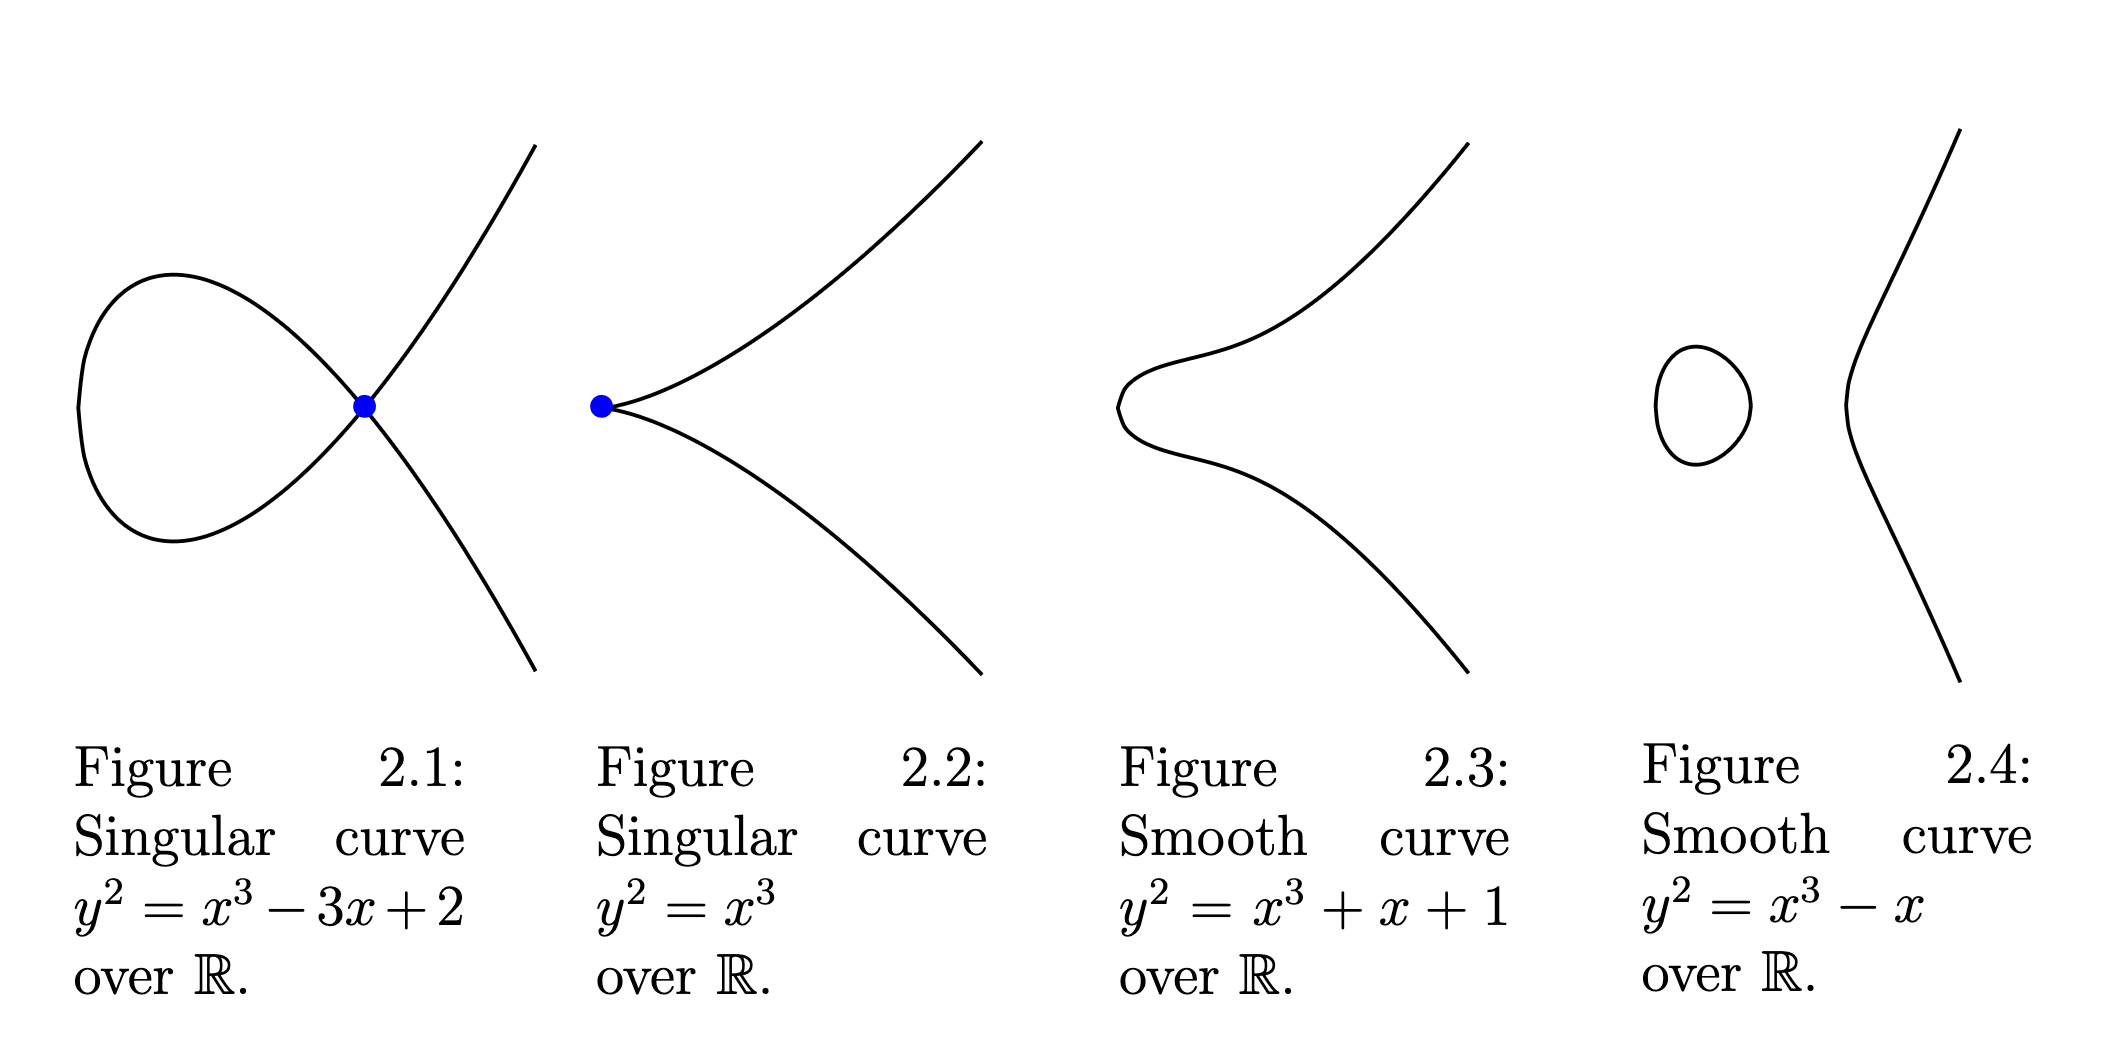
\includegraphics[width=0.9\textwidth]{resources/curves.png}
    \end{center}
    
\end{frame}

\begin{frame}{Еліптична крива над $\mathbb{C}$}
    Над полем комплексних чисел $\mathbb{C}$ еліптична крива є двоперіодичною мероморфною функцією, що топологічно еквівалентна тору (сфері із 1 ручкою, звідси рід(genus) кривої - 1)
    \begin{center}
    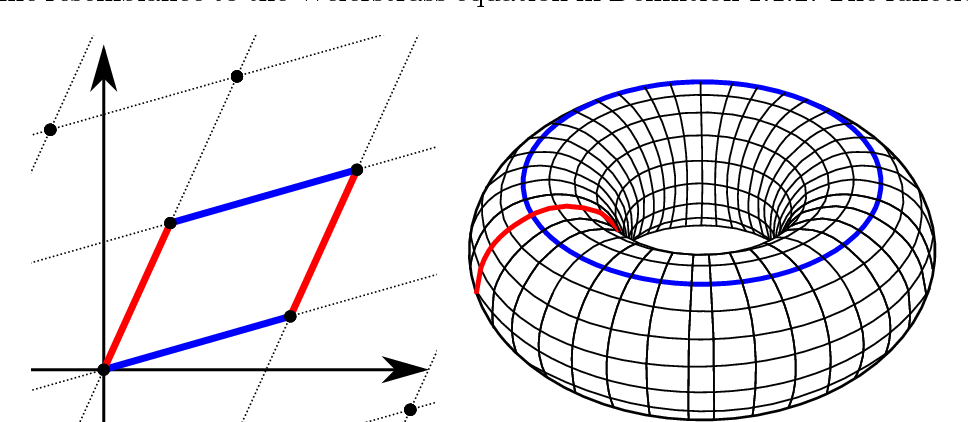
\includegraphics[width=0.9\textwidth]{resources/torus.png}
    \end{center}
    
\end{frame}

% Слайд 3: Означення еліптичної кривої
\begin{frame}{Означення еліптичної кривої}
\begin{block}{Еліптична крива над полем $K$}
Множина точок $(x,y) \in \overline{K}^2$, що задовольняють рівнянню:
\[
  E/K: y^2 + a_1 xy + a_3 y = x^3 + a_2 x^2 + a_4 x + a_6, \quad a_i \in K, \Delta \neq 0
  \]
  плюс точка на нескінченності $\mathcal{O}$
\end{block}
\begin{block}{Еліптична крива над полем $K, char(K) \neq 2,3$}
  Множина точок $(x,y) \in \overline{K}^2$, що задовольняють рівнянню Вейєрштраса:
  \[
  E/K: y^2 = x^3 + ax + b,\quad a,b\in K,\quad \Delta = 4a^3+27b^2\neq 0.
  \]
  плюс точка на нескінченності $\mathcal{O}$
\end{block}
\end{frame}

\begin{frame}{Група точок}
На початку XXст. Пуанкаре (1901) висловив ідею що $K$-раціональні точки кривої, координати яких належать полю $K$ утворюють групу(при цьому назвавши це не групою, а \textit{un système des points rationelles fundamentaux}). В 1922 Марделл довів теорему що група $K$-раціональних точок є скінченнопородженою абелевою групою.
\begin{block}{Теорема Марделла-Вейля}
Множина $E(K)$ $K$-раціональних точок еліптичної кривої $E/K$ утворює скінченнопороджену абелеву групу за операцією додавання точок із нейтральним елементом $\mathcal{O}$
\end{block}
\end{frame}

\begin{frame}{Додавання точок на кривій}
\begin{center}
    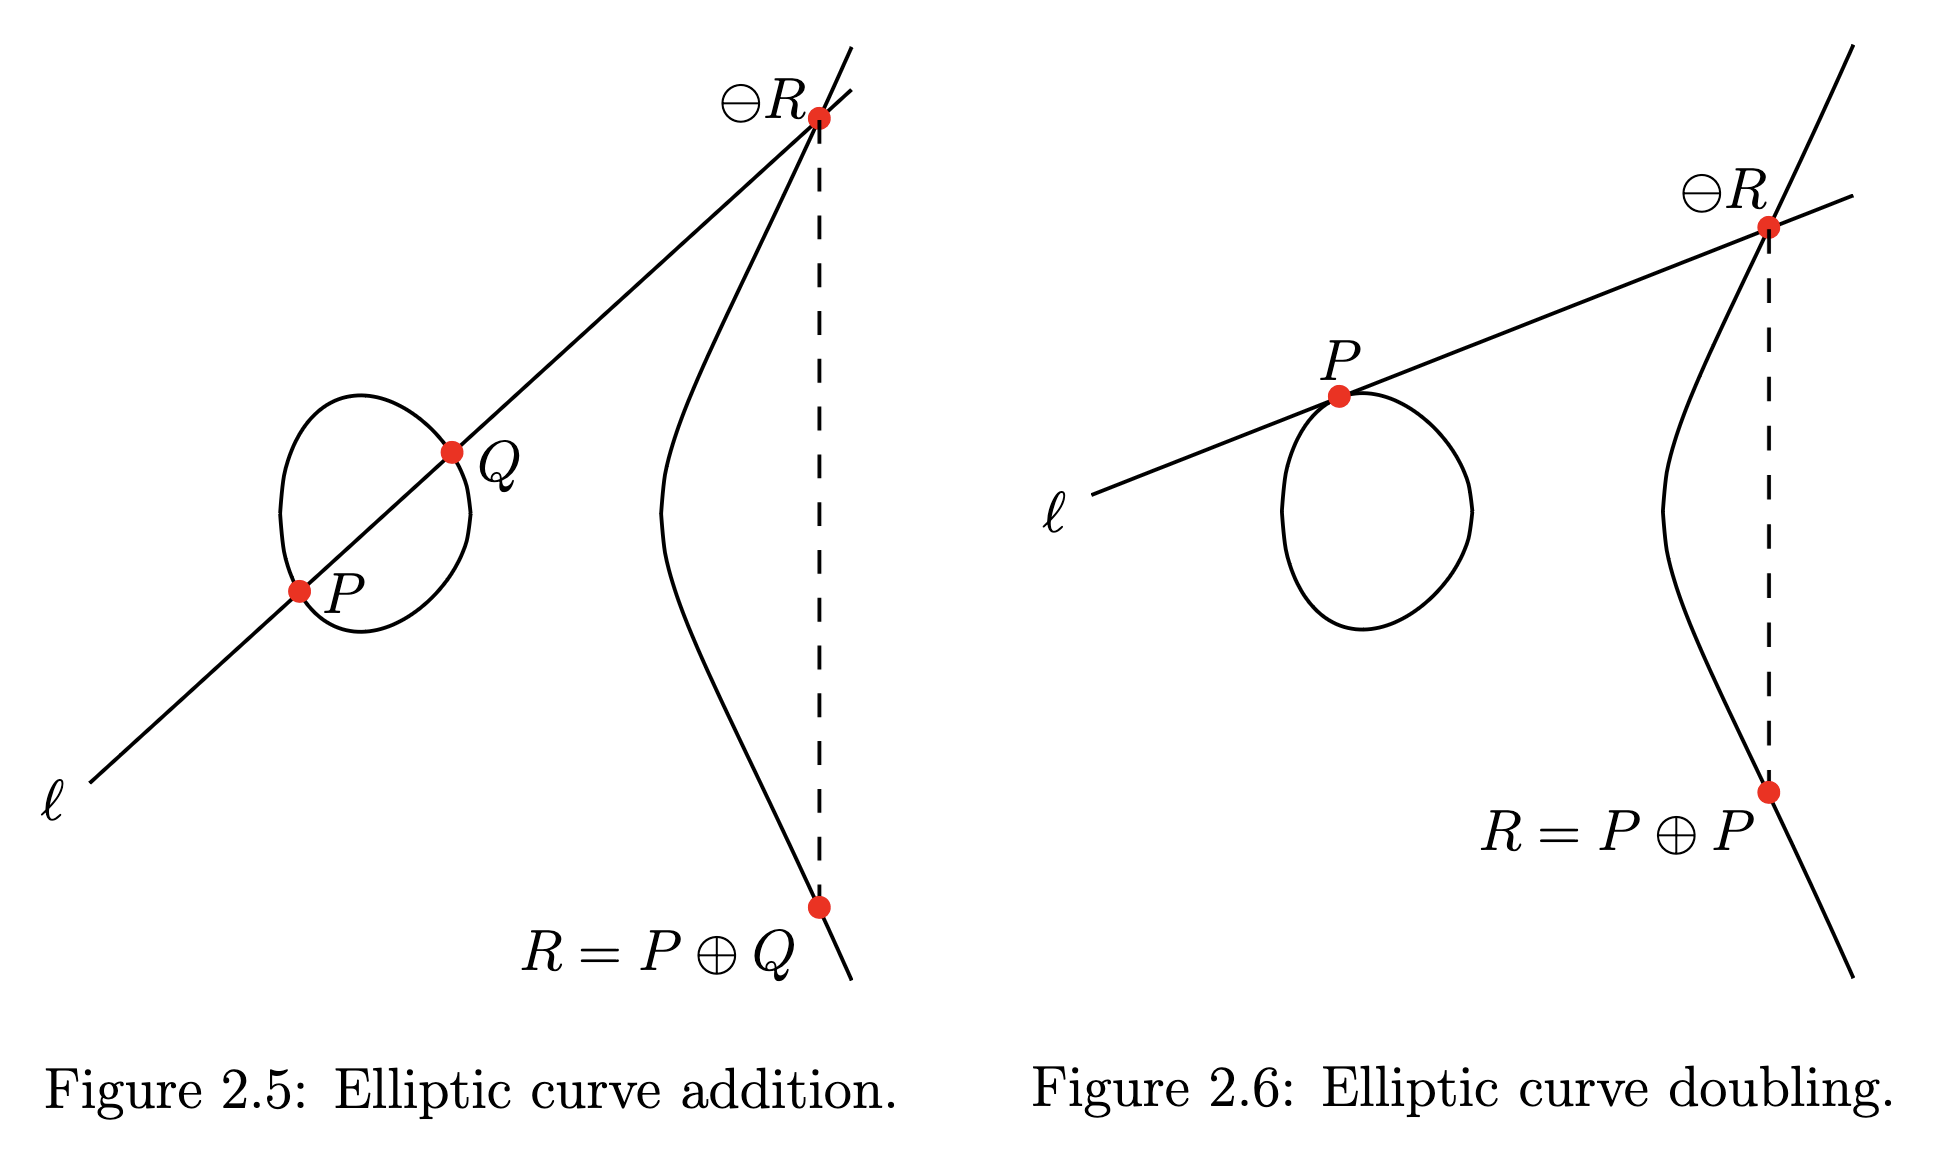
\includegraphics[width=0.9\textwidth]{resources/addition.png}
    \end{center}
\end{frame}

\begin{frame}{Група точок еліптичної кривої}
        \begin{block}{Груповий закон}
            \begin{enumerate}
                \item Точка на нескінченності $\mathcal{O}$ - нейтральний елементр. 
                \item Якщо $x_P\neq x_Q$, визначимо тангенс кута нахилу прямої між точками $\lambda := \frac{y_P-y_Q}{x_P-x_Q}$. Тоді точка $R=(x_R, y_R) = P \oplus Q$:
                \begin{equation*}
                    x_R := \lambda^2 - x_P - x_Q, \quad y_R := \lambda(x_P-x_R)-y_P.
                \end{equation*}
                \item Якщо $P=Q$, тоді тангенс кута нахилу дотичної в точці $P$ $\lambda := \frac{3x_P^2+a}{2y_P}$, при цьому $R=(x_R, y_R)=2P$:
                \begin{equation*}
                    x_R := \lambda^2 - 2x_P, \quad y_R := \lambda(x_P-x_R)-y_P.
                \end{equation*}
                \item Якщо $x_P = x_Q, y_P = -y_Q$, тобто $P=\ominus Q$ тоді $P \oplus Q := \mathcal{O}$.
            \end{enumerate}
        \end{block}
    \end{frame}
  \end{darkframes}




\end{document}
